% =====================================================================
%  Join ordering: four equivalent join trees for
%    SELECT * FROM R, S, T WHERE R.A = S.A AND S.B = T.B
%  after [L14, s.18]
%  Compile:  pdflatex join-orders.tex   (inside this folder)
%  Output:   join-orders.pdf  -> 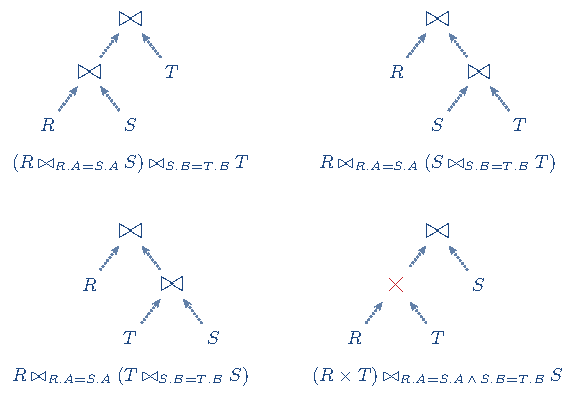
\includegraphics{join-orders}
% =====================================================================
\makeatletter\def\input@path{{../../theme/}}\makeatother   % shared palette
\documentclass[tikz,border=2pt,11pt]{standalone}
\usepackage[T1]{fontenc}
\usepackage[defaultsans]{lato}
\renewcommand{\familydefault}{\sfdefault}
\usepackage{amsmath,amssymb}
\usepackage{vinuni-palette}
\usetikzlibrary{arrows.meta}

\newcommand{\J}{\text{\Large$\bowtie$}}          % join node
\newcommand{\X}{\text{\Large$\times$}}           % cross-product node
\newcommand{\jn}[1]{\mathbin{\bowtie_{#1}}}      % join in a caption

\begin{document}
\begin{tikzpicture}[
    every node/.style={text=vinuNavy, font=\footnotesize},
    level distance=9mm, sibling distance=14mm,
    edge from parent/.style={draw=none},
    up/.style={-{Stealth[length=1.4mm]}, densely dotted, thick, vinuNavy!70},
    caption/.style={font=\footnotesize, text=vinuNavy}]

  % helper: dotted arrows from every child up to its parent (data flows upward)
  \tikzset{edge from parent path={}}

  % ---- (1) (R join S) join T  -------------------------------------
  \begin{scope}[xshift=0mm]
    \node (a) {$\J$}
      child { node (a1) {$\J$} child { node (a11) {$R$} } child { node (a12) {$S$} } }
      child { node (a2) {$T$} };
    \foreach \c/\p in {a1/a, a2/a, a11/a1, a12/a1} \draw[up] (\c) -- (\p);
    \node[caption] at (0,-24.5mm) {$(R \jn{R.A=S.A} S) \jn{S.B=T.B} T$};
  \end{scope}

  % ---- (2) R join (S join T)  -------------------------------------
  \begin{scope}[xshift=52mm]
    \node (b) {$\J$}
      child { node (b1) {$R$} }
      child { node (b2) {$\J$} child { node (b21) {$S$} } child { node (b22) {$T$} } };
    \foreach \c/\p in {b1/b, b2/b, b21/b2, b22/b2} \draw[up] (\c) -- (\p);
    \node[caption] at (0,-24.5mm) {$R \jn{R.A=S.A} (S \jn{S.B=T.B} T)$};
  \end{scope}

  % ---- (3) R join (T join S)  -------------------------------------
  \begin{scope}[yshift=-36mm]
    \node (c) {$\J$}
      child { node (c1) {$R$} }
      child { node (c2) {$\J$} child { node (c21) {$T$} } child { node (c22) {$S$} } };
    \foreach \c/\p in {c1/c, c2/c, c21/c2, c22/c2} \draw[up] (\c) -- (\p);
    \node[caption] at (0,-24.5mm) {$R \jn{R.A=S.A} (T \jn{S.B=T.B} S)$};
  \end{scope}

  % ---- (4) (R x T) join S  — has a cross product -------------------
  \begin{scope}[xshift=52mm, yshift=-36mm]
    \node (d) {$\J$}
      child { node (d1) {\textcolor{vinuRed}{$\X$}} child { node (d11) {$R$} } child { node (d12) {$T$} } }
      child { node (d2) {$S$} };
    \foreach \c/\p in {d1/d, d2/d, d11/d1, d12/d1} \draw[up] (\c) -- (\p);
    \node[caption] at (0,-24.5mm) {$(R \times T) \jn{R.A=S.A \,\wedge\, S.B=T.B} S$};
  \end{scope}
\end{tikzpicture}
\end{document}
